\documentclass{article}

% Set the margins of the page.
\usepackage[a4paper, total={6.5in, 9in}]{geometry}

% A bunch of math packages.
\usepackage{amssymb}
\usepackage{amsmath}
\usepackage{amsthm}
\usepackage{amsfonts}
\usepackage{mathtools}
\usepackage{float}

\usepackage{changepage}
\usepackage{graphicx} 		% Insert images
\usepackage{color}				% COLORS!
\usepackage[shortlabels]{enumitem}			% More enumerate types such as \alph*
\usepackage{listings}			% Used for code-blocks in latex.
\usepackage{hyperref}

% Create links when using ref and table of contents.
\hypersetup{colorlinks=true, linkcolor=black}

% Replace the indents for paragraphs with empty lines.
\usepackage[parfill]{parskip}

\usepackage[myheadings]{fancyhdr}
\usepackage{titleref}
\makeatletter
\newcommand*{\currentname}{\TR@currentTitle}
\makeatother

% Number equations with reference to sub sections.
\numberwithin{equation}{subsection}

\definecolor{lightgray}{RGB}{200, 200, 200}

% Set some style rules for code-blocks
\lstset{
	literate={<-}{$\leftarrow$}{2} {\\infty}{$\infty$}{1},
	backgroundcolor=\color{lightgray}
,
	framexleftmargin=2pt,
	framexrightmargin=2pt,
	framextopmargin=2pt,
	framexbottommargin=2pt,
	frame=single,
	basicstyle=\fontsize{10pt}{15pt}\selectfont,
	stepnumber=1,
	tabsize=4,
}


%increases table padding
\def\arraystretch{1.5}



\title{\textbf{CSCI-2201\\Lab-3}}
\author{Anas Alhadi\\B00895875}


\begin{document}

	\maketitle
	
	\section{Exercise 1}
	\subsection{HTTP GET vs POST}

	\par{
		Both GET and POST are HTTP request methods used to indicate the purpose of the
		request. GET requests are used to retrieve a resource from the server (aka a file), without
		changing state (so the resource is unchanged in the server). 
	}

	\par{
		On the other hand, POST requests are used to send data to the server with the purpose
		of updating a resource (or creating one of the specified resource does not exist), unlike GET
		requets, a POST changes the server's state, such that duplicated POSTS can
		result in different effect/responses (2 duplicated GET requets will always have the same response).
	}

	\subsection{TCP stream}
	\begin{figure}[H]
		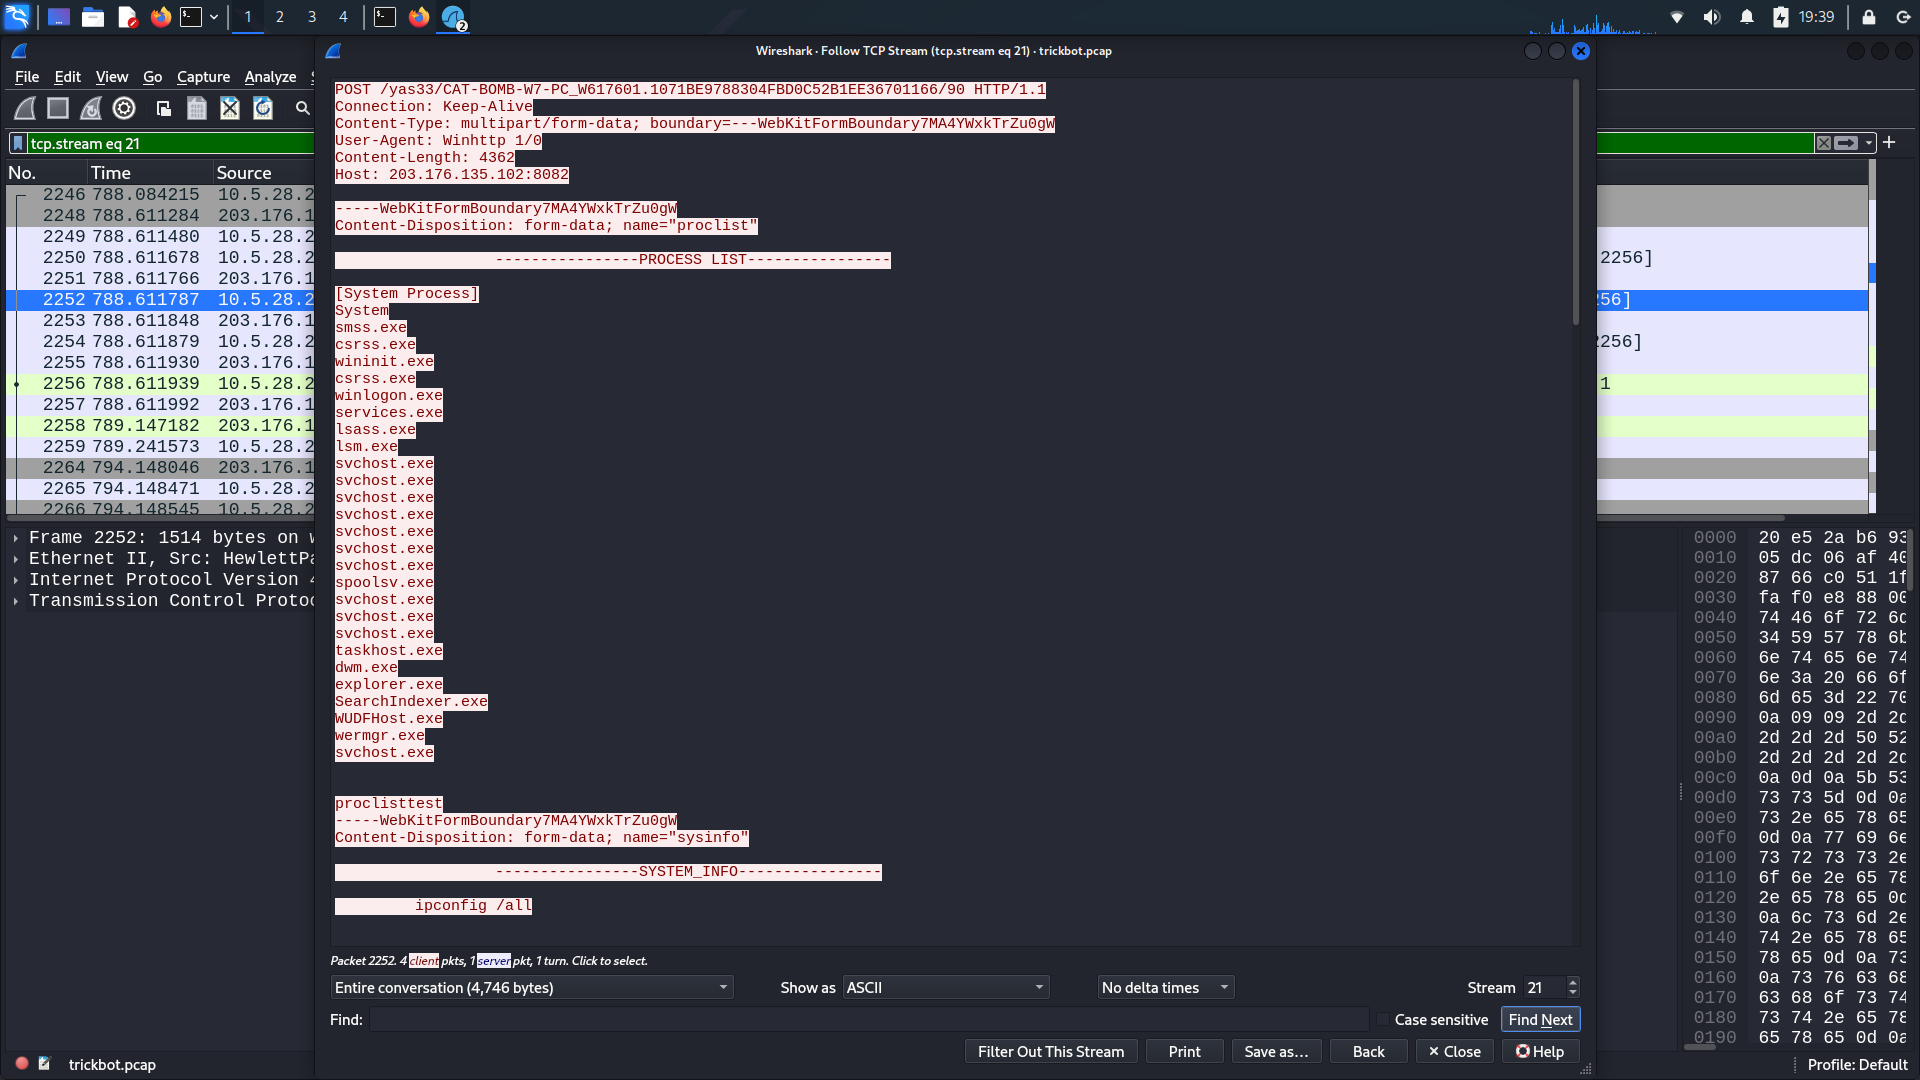
\includegraphics[width=400pt]{pics/1.png}
	\end{figure}

	\begin{itemize}
		\item \textbf{HOST NAME:} Cat-Bomb-W7-PC
		\item \textbf{DOMAIN NAME:} catbomber.net
	\end{itemize}

	\newpage

	\section{Exercise 2}
	\subsection{TCP stream}
	\begin{figure}[H]
		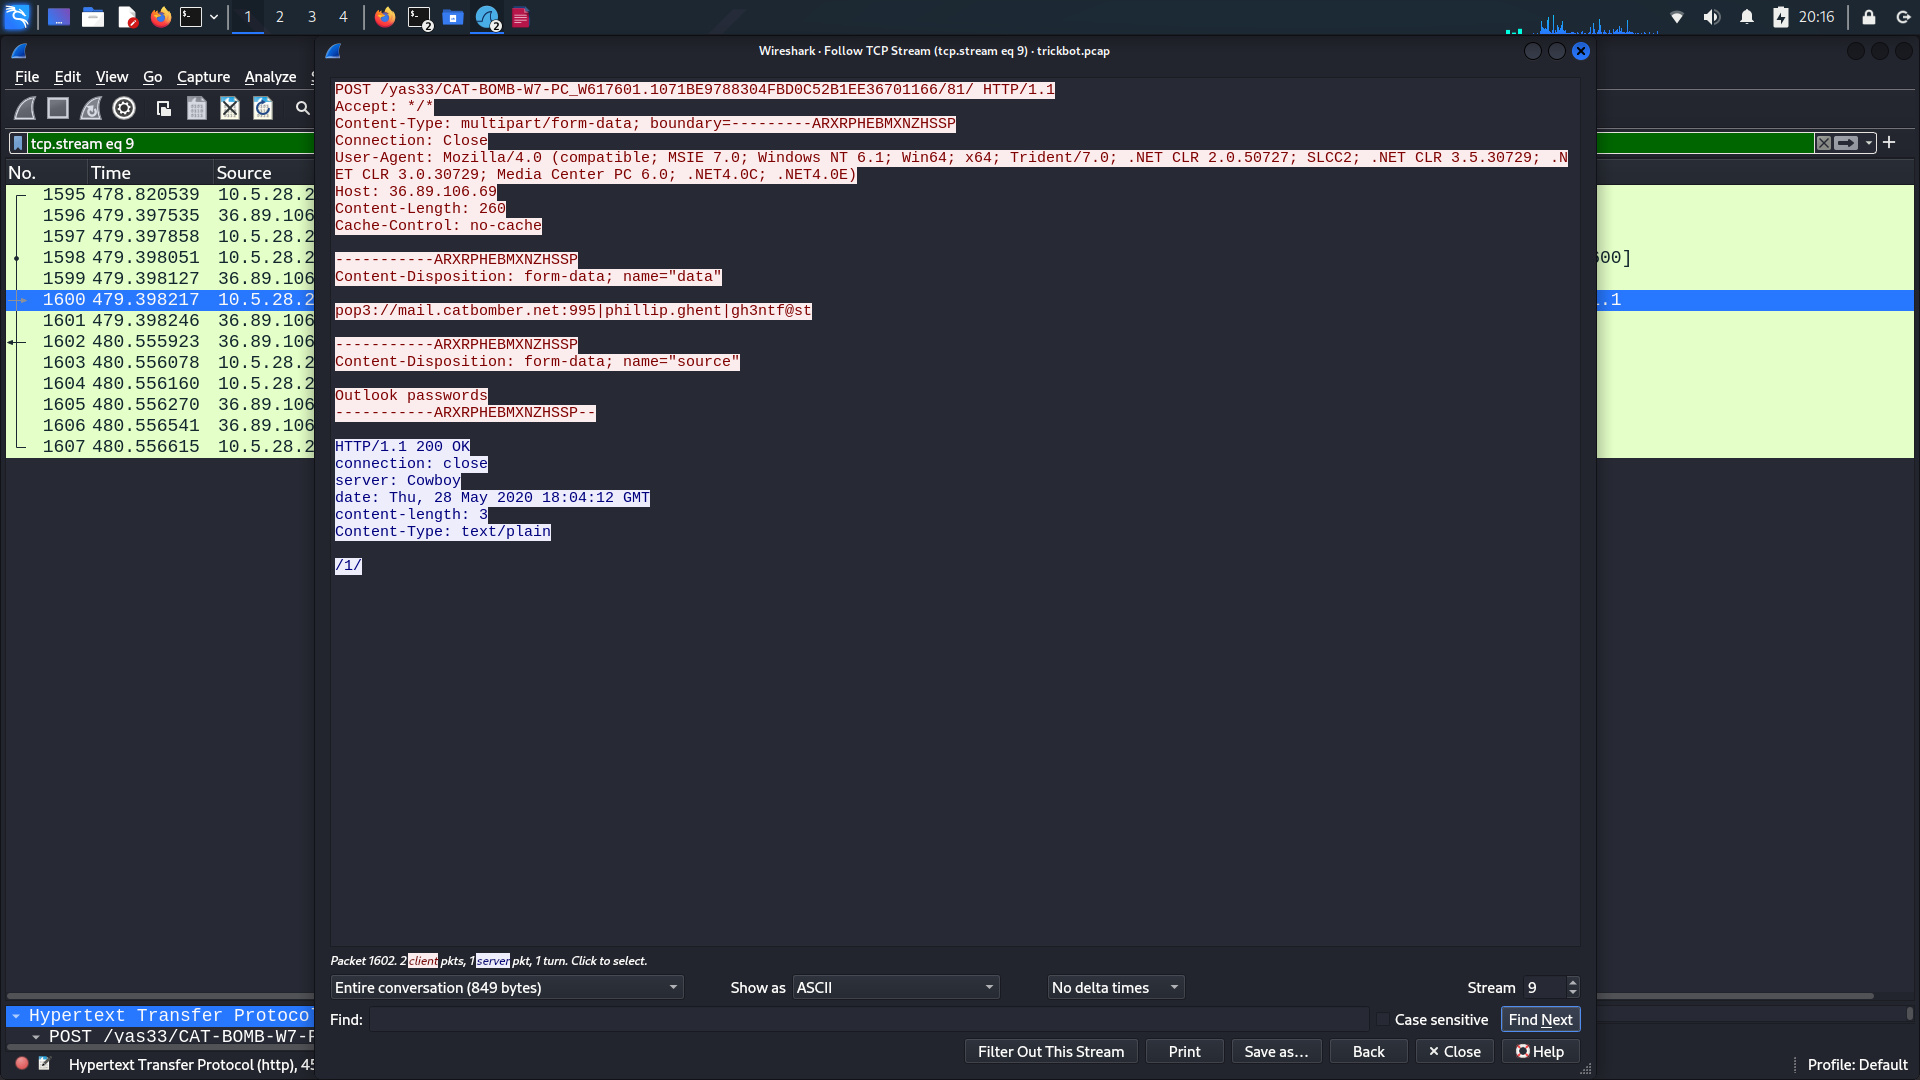
\includegraphics[width=400pt]{pics/2.png}
	\end{figure}


	\begin{itemize}
		\item \textbf{Email:} phillip.ghent@mail.catbomber.net
		\item \textbf{Password:} gh3ntf@st
	\end{itemize}

	\newpage
	\section{Exercise 3}
	\par{
		The attacker disguises the executable files as .png files
	}	


	\vspace{30pt}
	\section{Exercise 4}

	\subsection{Prevention:}
	\par{
		Stricter policies need to be defined regarding the interaction with any 
		external emails and to avoid pressing on any links. Spam detection frameworks 
		should also be used to reduce the amount of such emails that reach the users.
	}

	\subsection{Protection:}
	\par{
		Once a device have been identified to have been infected with malware, it needs
		to be immediately disconected from the network.
	}
\end{document}
